% Chapter 1
\setstretch{1.8}
\chapter{Introduction} % Write in your own chapter title
\label{Chapter1}
\lhead{Chapter 1. \emph{Introduction}} % Write in your own chapter title to set the page header

\section{Background}

Electric motors are an important invention of the modern era and comprise a major portion of the electric load of any country. Induction motors are the most commonly used type of motors, being used widely in industry, agriculture, domestic, municipal and commercial applications. In a domestic environment, they are found in many appliances, including but not limited to air conditioners, refrigerators, water pumps, and kitchen appliances (grinder, blender, etc.). In agriculture they are used as pumps, for watering the crops. In industry, they are found at different places according to the nature of industry, e.g. in textiles, they are using in weaving mills, in oil and gas, they are used in pumps, in assembly line, they are used to drive the belts, etc. According to the WEC (World Energy Council), in industrialized countries three main sectors are responsible for three quarters of electricity consumption: electric motors, 45 \%, lighting, about 15 \%, and home appliances and consumer electronics, also around 15 \%.Global energy consumption of electric motors is around 9000 TWh per year. These data show the impact that electric motors produce on electrical energy consumption. Therefore, the manufacturers in this sector are investing heavily in the energy efficiency of their products. The following figures show the statistical usage of electric machines [INSERT PIE CHARTS AND GRAPHS HERE].

\section{Switching to an efficient world}
From the above scenario, it is clear that induction machines comprise a major part of the total electric load of any country. So, the efficiency of these motors is an important parameter in controlling the total load. If the machines are replaced by more efficient ones, a large amount of energy can be saved.
\begin{figure}[htbp]
  \centering
    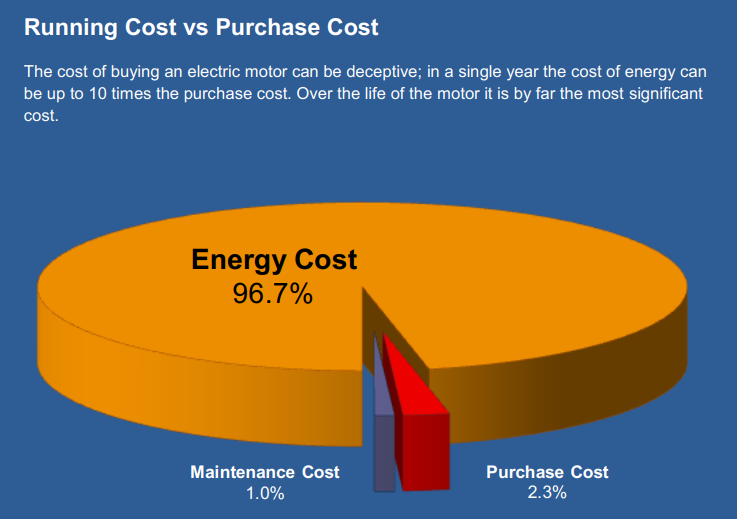
\includegraphics[width = 5in]{./Figures/MS/fig11.png}
    \rule{35em}{1.2pt}
  \caption{Running cost vs purchase cost of induction motors}
  \label{fig:Running cost vs purchase cost of induction motors}
\end{figure}
\begin{figure}[htbp]
  \centering
    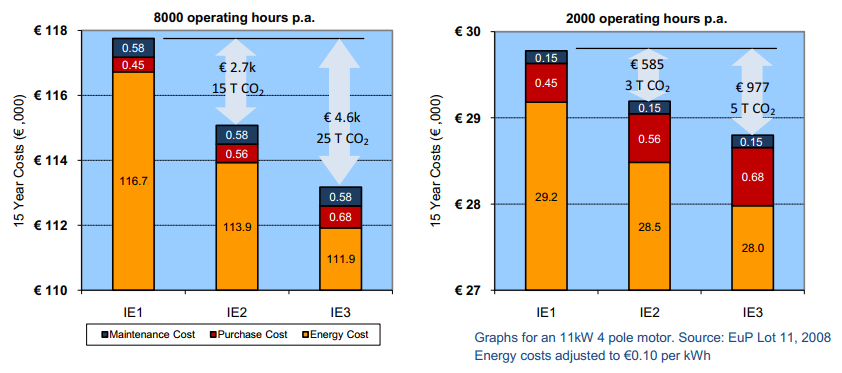
\includegraphics[width = 5in]{./Figures/MS/fig12.png}
    \rule{35em}{1.2pt}
  \caption{Cost comparison of IE1, IE2 and IE3 motors}
  \label{fig:Cost comparison of IE1, IE2 and IE3 motors}
\end{figure}
At 8000 operating hours per year, the additional cost of an IE2 motor is paid back in 7 months, with an IE3 motor paying back in 10 months. Even at only 2000 operating hours per year, the energy saving repays the capital in about 3 years.

\section{Domestic Use of Motors in Pakistan}
Motors are found in Pakistan in almost all the homes for water supply. This thesis particularly focuses on these motors. There are two main types of motor pumps available in the market:
\begin{itemize}
	\item Reciprocating pumps
	\item Centrifugal pumps
\end{itemize}
Reciprocating pumps are being used more while centrifugal pumps have recently entered the domestic market. They were previously commonly used in large setups like tube wells and municipal pumps.
\begin{figure}[htbp]
  \centering
    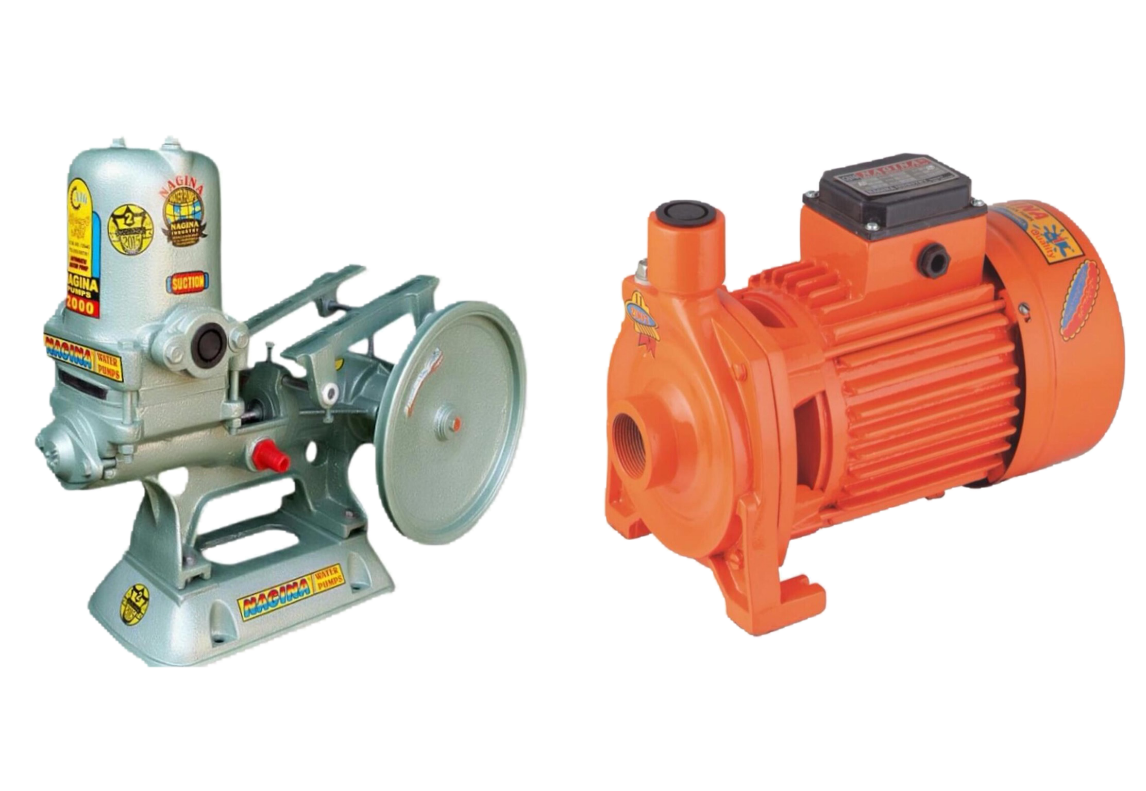
\includegraphics[width = 5in]{./Figures/MS/fig13.png}
    \rule{35em}{1.2pt}
  \caption{Reciprocating pump(left) vs Centrifugal pump(right)}
  \label{fig:Reciprocating pump(left) vs Centrifugal pump(right)}
\end{figure}
The local market in Pakistan for domestic motor pumps has not been following any international standards. IEC endorsed its efficiency standards to Pakistan in 2017, which has opened new opportunities for the manufacturers to use improved testing methods and identify the possible causes of losses and efficiency and improve them. This thesis also focuses on utilizing the IEC standards to create a standardized test bench which can be made available in the local market for low costs. Currently, such setups cost around 25,000 USD for setups with capacity to test 10 hp motors. 

\section{Objectives}
The main goal of the project was to develop a test bench for evaluating the efficiency of small induction motors simular to those used in domesting water pumping applications. This work of this project will be extended to design test benches that will be used to evaluate the efficiences of the motors available in the Pakistan local market, under the HEC TDF-02-173 project, which aims at development of a testbench for motor/pump strings so they can be tested and certified according to international standards. This project is also a part of the HEC project.
\begin{figure}[htbp]
  \centering
    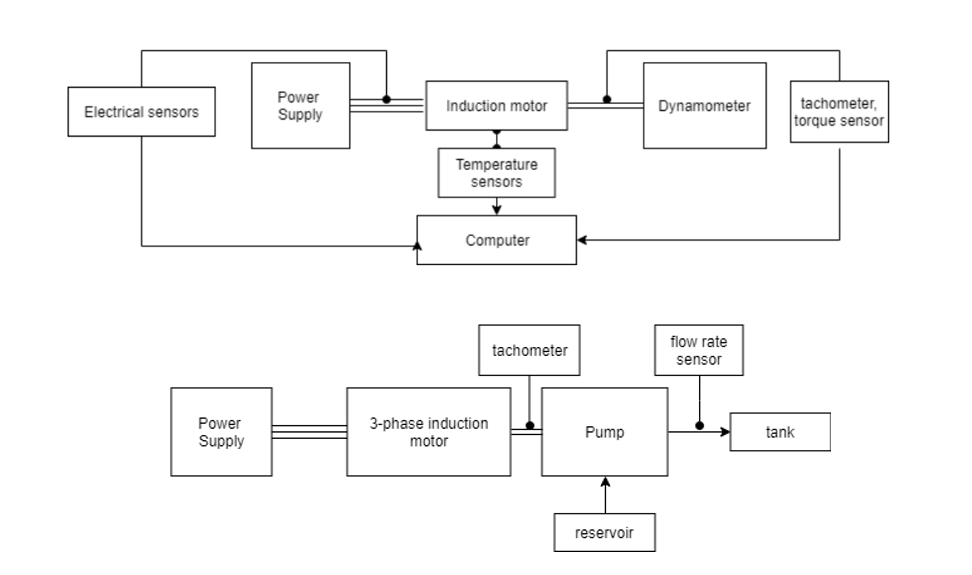
\includegraphics[width = 5in]{./Figures/MS/fig16.png}
    \rule{35em}{1.2pt}
  \caption{Scope of the HEC TDF-02-173 project.}
  \label{fig:Scope of the HEC TDF-02-173 project.}
\end{figure}
\begin{figure}[htbp]
  \centering
    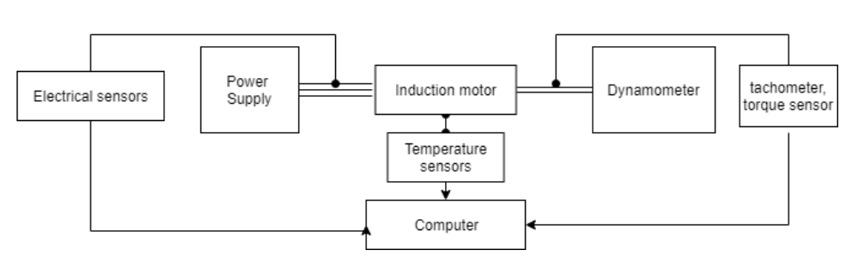
\includegraphics[width = 5in]{./Figures/MS/fig17.png}
    \rule{35em}{1.2pt}
  \caption{Scope of this thesis project.}
  \label{fig:Scope of this thesis project.}
\end{figure}

\section{MEPS (Minimum Energy Performance Standards)}
MEPS is a set of policies in a country that defines minimum efficiencies for different appliances and machinery sold in that country. This trend was started by the USA with the energy policy act of 1992, in which a large number of machines were required to be upgraded to comply with the efficiency standards. This policy was implemented in 8 years, in different phases. Europe followed and the CEMEP (European Committee of Manufacturers of Electrical Machines and Power Electronics) also created a similar policy. Currently, the minimum efficiency requirements in the USA are IE3, while EU allows IE3 or IE2 motors with a VFD as it has increased efficiency. These efficiency classes are defined by the IEC 60034-30-1 standard. Some other countries that have also defined MEPS for a set of appliances e.g. Air Conditioners, Refrigerators, lighting equipment, etc. include, but not limited to, Australia, Brazil, Japan, China, New Zealand.   
In Pakistan, the National Energy Efficiency \& Conservation Authority (NEECA) is responsible for maintaining energy standards. Currently, it has defined rules for air conditioners, refrigerators, fluorescent bulbs and induction motors. For induction motors, since the standards have recently been applied, so the efficiency requirements are set a bit lower than international standards so allow the local manufacturers to catch up. e.g. the required minimum efficiency for an IE1 4-pole 50 Hz motor is 66 \%, while NEECA has set it to 62.7 \% for its phase-1.
\begin{figure}[htbp]
  \centering
    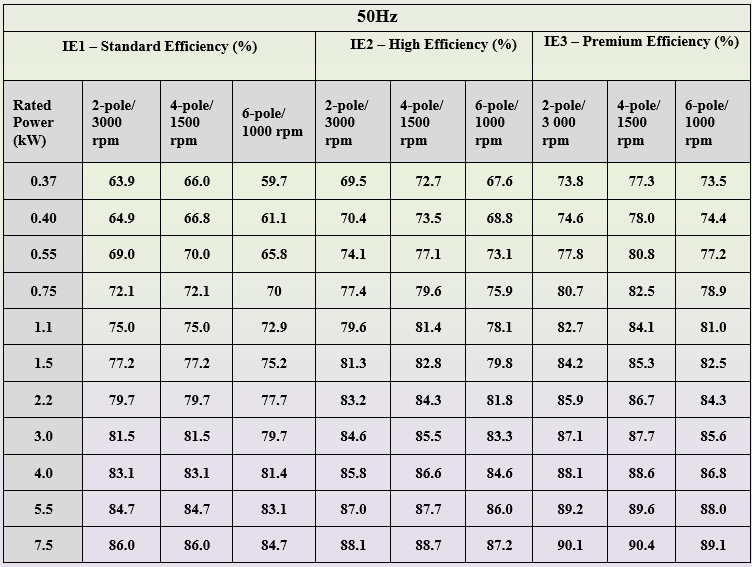
\includegraphics[width = 5in]{./Figures/MS/fig14.png}
    \rule{35em}{1.2pt}
  \caption{Minimum efficiencies for induction motors by IEC-60034-30}
  \label{fig:Minimum efficiencies for induction motors by IEC-60034-30}
\end{figure}
\begin{figure}[htbp]
  \centering
    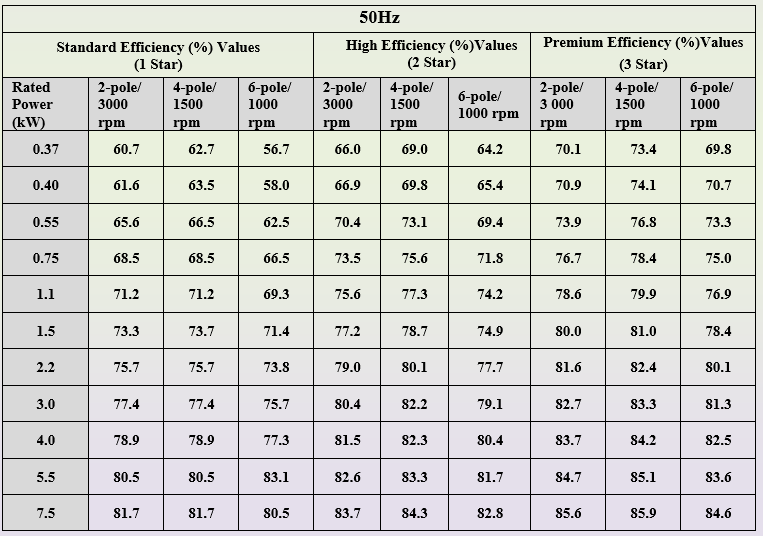
\includegraphics[width = 5in]{./Figures/MS/fig15.png}
    \rule{35em}{1.2pt}
  \caption{Modified minimum efficiencies for induction motors by NEECA}
  \label{fig:Modified minimum efficiencies for induction motors by NEECA}
\end{figure}

\section{Thesis Outline}
Chapter 2 of the thesis provides a brief overview of the literature behind the losses in the machines. Losses are categorized according to the IEC standard and another section that introduces the factors in machines that mainly cause these losses.
Chapter 3 gives and introduction to machine testing and also discusses the techniques used in this project. It also provides a provides the market estimated prices and quotations for the different types of sensors required for making a hardware setup
Chapter 4 is related to the algorithms, codes and flowcharts for the strategies used. The project was completely simulated in MATLAB and Simulink, where physical systems were designed in Simulink and algorithms were implemented using MATLAB scripts
Chapter 5 provides the results of the different tests performed and concluding remarks.
